\documentclass[a4paper,11pt]{article}
\usepackage[T1]{fontenc}
\usepackage[utf8]{inputenc}
\usepackage{lmodern}
\usepackage[francais]{babel}
\usepackage{geometry}
\usepackage{graphicx}
\usepackage{amsmath}
\usepackage{amssymb}
\usepackage{mathrsfs}
\usepackage{listings,color}

\definecolor{verbgray}{gray}{0.9}

\lstnewenvironment{code}{%
  \lstset{backgroundcolor=\color{verbgray},
  frame=single,
  framerule=0pt,
  basicstyle=\ttfamily,
  columns=fullflexible}}{}

\definecolor{shadecolor}{rgb}{.9, .9, .9}
\geometry{hmargin = 2.5cm, vmargin = 1.5cm}

\title{SY09 - TP02\\Analyse factorielle d’un tableau de distances,classification automatique}
\author{Félix Flores - Cristian Garrido}
\begin{document}

\maketitle
%asjhgajhgskjhagshgashgaksjhgahsjgahsjgakjhsgahsg

\section{Analyse factorielle d’un tableau de distances}
On considère le tableau de données suivant \textit{X} la matrice de données et $X_{c}$ la matrice \textit{X} centrée:
\[X = \begin{pmatrix}
8.5 & 3.5 \\
2.0 & 9.5 \\
8.5 & 3.0 \\
9.0 & 2.0 \\
1.5 & 5.0 \\
6.5 & 1.5 \\
2.5 & 6.5 \\
2.5 & 5.5 \\
\end{pmatrix},
X_{c} = \begin{pmatrix}
2.75 & -2.4375\\
-2.25 & 1.0625\\
-3.75 & 2.5625\\
3.75 & -2.4375\\
2.75 & -1.4375\\
-2.75 & 2.5625\\
3.25 & -1.4375\\
-3.75 & 1.5625
 \end{pmatrix}\]
\\
\begin{enumerate}
  \item Calculer le tableau $D^2$ des distances euclidiennes associé à ces données.
    \[D^2 = \begin{pmatrix}
    0 \\
    37.25 & 0 \\
    67.25 & 4.50 & 0 \\
    1 & 48.25 & 81.25 & 0 \\
    1 & 31.25 & 58.25 & 2 & 0 \\
    55.25 & 2.50 & 1 & 67.25 & 46.25 & 0 \\
    1.25 & 36.50 & 65 & 1.25 & 0.25 & 52 & 0 \\
    58.25 & 2.50 & 1 & 72.25 & 51.25 & 2 & 58 & 0
    \end{pmatrix}\]
    
  \item Calculer la matrice $W$ des produits scalaires : d’une part directement à partir de $X$, d’autrepart à partir de $D^2$.\\
    \[W =\begin{pmatrix}
    13.50 & -8.78 & -16.56 & 16.25 & 11.07 & -13.81 & 12.44 & -14.12\\
    -8.78 &  6.19 & 11.16 & -11.03 & -7.71 &  8.91 & -8.84 & 10.10\\
    16.56 & 11.16 & 20.63 & -20.31 & -14.00 & 16.88 & -15.87 & 18.07\\
    16.25 & -11.03 & -20.31 & 20.00 & 13.82 & -16.56 & 15.69 & -17.87\\
    11.07 & -7.71 & -14.00 & 13.82 &  9.63 & -11.25 & 11.00 & -12.56\\
    13.81 &  8.91 & 16.88 & -16.56 & -11.25 & 14.13 & -12.62 & 14.32\\
    12.44 & -8.84 & -15.87 & 15.69 & 11.00 & -12.62 & 12.63 & -14.43\\
    14.12 & 10.10 & 18.07 & -17.87 & -12.56 & 14.32 & -14.43 & 16.50
    \end{pmatrix}\]\\
    Après d'avoir calculé des deux façons, nous avons obtenu le même résultat. Nous pouvons alors constater que l'égalité $W = XX'= -\frac{1}{n}Q_{n}X_{c}Q_{n}$ est validé.\\
    
    
    \item Vérifier que $W$ (ou $\frac{1}{n}W$ ) est semi définie positive.\\
    Pour vérifier si $W$ est semi définie positive, il faut constater si ses valeurs propres sont positives.
    Après ce calcul, Cinq valeurs sont positives et trois sont négatives. Cependant nous avons obtenu deux valeurs positives dont est concentrés presque la totalité de l'information. Par ailleurs, nous avons noté que les 3 valeurs négatives et les autres deux positives sont très proches à 0 (< $10^{-15}$). Ces valeurs donc nous les avons considérées comme 0.
    Le fait que $W$ soit une matrice produits scalaires positives ou nuls nous indique que $W$ est donc semi-définie positive. On sait d'ailleurs que $\frac{1}{n}>0$ alors  $\frac{1}{n}W$ sera SDP aussi.\\
    
    
    \item Déterminer la matrice $\varLambda$ des vecteurs propres (normés au sens de $D_p$ ) de $\frac{1}{n}W$ et $L$ la matrice diagonale des valeurs propres.\\
    \[\varLambda = \begin{pmatrix}
        0.34 & 0.46 & 0.00 & 0.82 & 0.00 & 0.00 & 0.00 & 0.00\\
        0.23 & 0.22 & -0.91 & -0.03 & 0.10 & 0.08 & -0.02 & 0.24\\
        0.43 & -0.13 & 0.10 & 0.25 & -0.54 & -0.33 & 0.33 & 0.46\\
        0.42 & 0.05 & 0.07 & -0.21 & 0.43 & -0.46 & 0.14 & 0.59\\
        0.29 & -0.18 & -0.14 & -0.02 & 0.00 & 0.34 & 0.86 & -0.11\\
        0.35 & -0.54 & 0.01 & 0.44 & 0.63 & -0.02 & 0.03 & -0.02\\
        0.33 & -0.38 & -0.37 & 0.07 & -0.22 & -0.60 & -0.07 & -0.42\\
        0.38 & 0.50 & 0.09 & -0.12 & 0.26 & -0.43 & 0.37 & -0.44
    \end{pmatrix}\]
    \[ L = \begin{pmatrix}
      13.93 & 0 & 0 & 0 & 0 & 0 & 0 & 0\\
      0 & 0.22 & 0 & 0 & 0 & 0 & 0 & 0\\
      0 & 0 & 0 & 0 & 0 & 0 & 0 & 0\\
      0 & 0 & 0 & 0 & 0 & 0 & 0 & 0\\
      0 & 0 & 0 & 0 & 0 & 0 & 0 & 0\\
      0 & 0 & 0 & 0 & 0 & 0 & 0 & 0\\
      0 & 0 & 0 & 0 & 0 & 0 & 0 & 0\\
      0 & 0 & 0 & 0 & 0 & 0 & 0 & 0
    \end{pmatrix}\]\\

    \item En déduire la représentation multidimensionnelle fournie par l’AFTD.\\
    Nous avons déduite la représentation avec l'expression des composante principales $C=V\sqrt{L}$\\

    \item Tracer le nuage associé au tableau initial $X$ et le nuage associé à la représentation fournie par l’AFTD ; comparer ces deux représentations.\\
    \begin{center}
      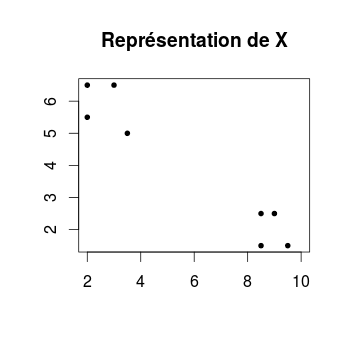
\includegraphics[height = 6cm, width = 6cm]{plots/1-6_repX.png}
      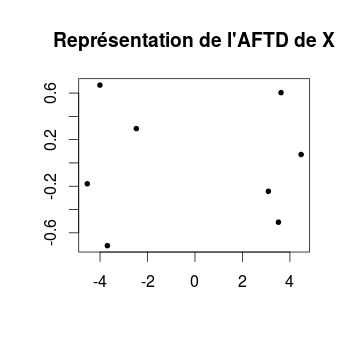
\includegraphics[height = 6cm, width = 6cm]{plots/1-6_repAFTD.png}
    \end{center}
    Nous avons constaté sur les graphiques qu'on a deux groupes bien identifiés. Et on peut voir aussi que dans la représentation de l'AFTD les distances entre les points de chaque groupe ont bien été réduits sur l'axe vertical.\\
    
    \newpage
    \item En utilisant les résultats précédents, écrire en R la fonction aftd ayant comme argument d’entrée la distance D et comme argument de sortie la représentation multidimensionnelle calculée par l’AFTD ainsi que la qualité de cette représentation.\\

      \begin{code}
        aftd <- function (distances, k=2) {
          D2 = as.matrix(distances)^2
          n = dim(D2)[1]
          In = diag(n)
          Un = matrix(rep(1, n^2), n)
          Qn = In - (1/n)*Un
          W = -(1/2)*Qn%*%D2%*%Qn
          
          V = eigen((1/n)*W)$vectors
          V = sqrt(n)*V[,1:k]
          
          L_ = eigen((1/n)*W)$values;
          L = diag(L_[1:k])
          
          result = NULL
          result$quality = (sum(abs(L))/sum(abs(diag(L_)))*100
          result$C <- V%*%sqrt(L)
          return(result)
        }
      \end{code}
      Cette fonction prend facultativement un paramétré \textit{k} pour négliger les valeurs propres trop petites 
\end{enumerate}
\subsection{Données de mutations.}
Dans cet exercice nous nous sommes servis de la base de données \textit{mutations2.txt} qui contienne un tableau de distances euclidiennes entre différents individus.
Ci-dessous nous avons fait une comparative entre la fonction \textit{aftd()} crée dans l'exercice précédant versus la fonction \textit{cmdscale()} du logiciel R.
    \begin{center}
      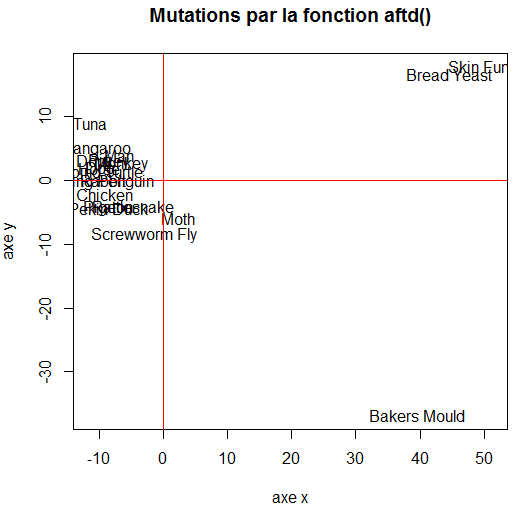
\includegraphics[height = 6cm, width = 6cm]{plots/1-1-1_mutation.png}
      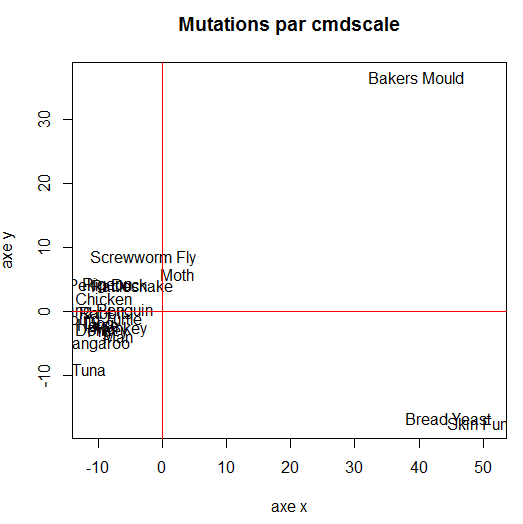
\includegraphics[height = 6cm, width = 6cm]{plots/1-1-2_mutation.png}
    \end{center}
Premièrement, dans la graphique de la fonction \textit{aftd()} nous pouvons noter que la nuage de données se concentre sur le deuxième et troisième quadrant du plan. Ceux-ci sont trouvés principalement sur le deuxième quadrant. Aussi nous pouvons remarquer que les individus \textit{Bakers Mould, Bread Yeast} et \textit{Skin Fungus} sont les plus éloignés de la nuage.\\
Concernant à la graphique de la fonction \textit{cmdscale()} nous avons trouvé une représentation des donnés similaire sur le plan. Cela par rapport à la nuage des individus où on trouve concentré la majorité des données. Nous avons aussi remarqué que les valeurs de cette graphique son identiques, celles changent au niveau d'axe vertical, c'est-à-dire, celles-ci sont équivalentes à l’antérieur mais multiplié par -1.\\
Maintenant, nous avons effectué l'AFTD utilisant des nombres de variables de représentation $k$ allant de 2 à 5. 
En ce que concerne à cet analyse, nous avons utilisé la fonction \textit{Shepard} pour tracer la graphique des résultats de la matrice de distances au tant aussi les résultats des donnés de mutation qui ont été traités avec la fonction \textit{cmdscale()} 
    \begin{center}
      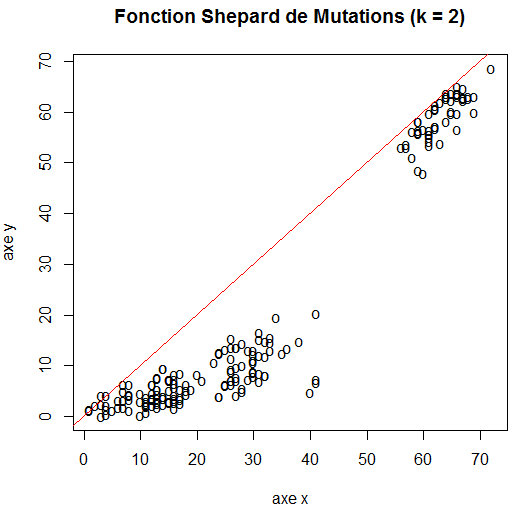
\includegraphics[height = 4cm, width = 3.8cm]{plots/1-2-1_mutation.png}
      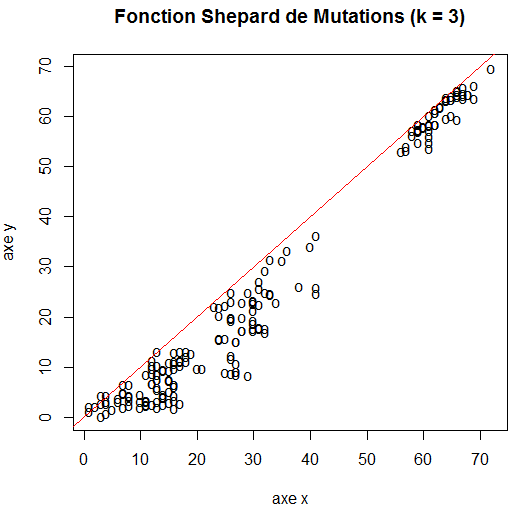
\includegraphics[height = 4cm, width = 3.8cm]{plots/1-2-3_mutation.png}
      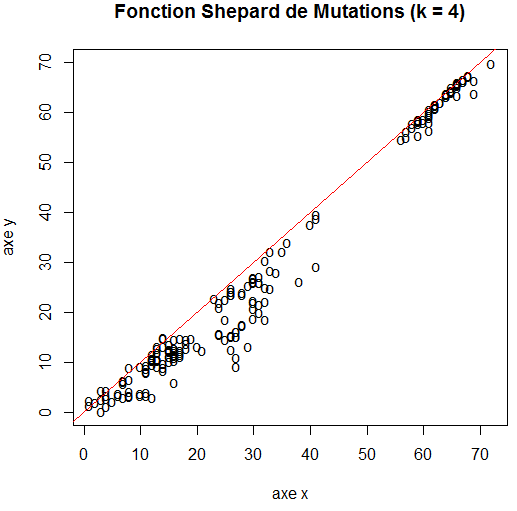
\includegraphics[height = 4cm, width = 3.8cm]{plots/1-2-4_mutation.png}
      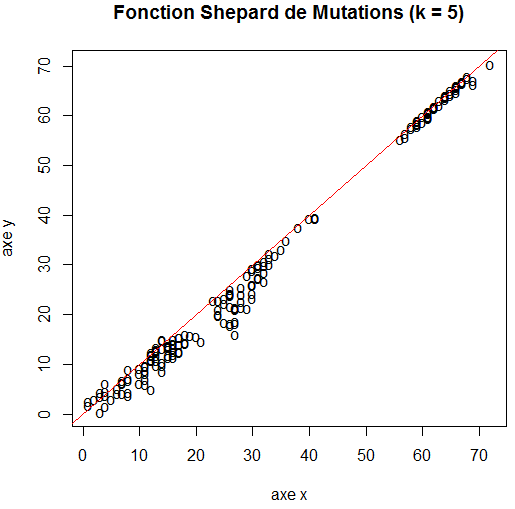
\includegraphics[height = 4cm, width = 3.8cm]{plots/1-2-5_mutation.png}
%      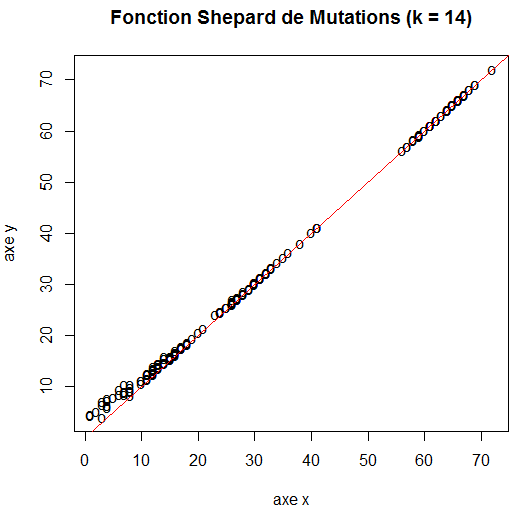
\includegraphics[height = 3.7cm, width = 5cm]{plots/1-2-6_mutation.png}
      \begin{tabular}{|c|c|c|c|c|}
      \hline
       & $k=2$ & $k=3$ & $k=4$ & $k=5$ \\
      \hline
      Qualité & 68.72455\% &  79.66872\% & 86.38446\% & 91.16358\% \\
      \hline
      \end{tabular}
    \end{center}
    Sur les graphiques nous avons tracé une droite ($y=x$) tels que les résultats soient plus facilement lisibles. Dans chaque graphique on peut trouver le changes du nuage au fur et à mesure que nous avons changé la valeur de $k$. Lorsque la valeur de $k$ va augmentant, nous pouvons constater une notable rapprochement du nuage des donnés par rapport à la droite tracé. Cela va toujours en augmente direct avec $k$ et cela nous assure aussi une fidélité des données.
Finalement, nous avons assigné la valeur $k=14$ et nous avons obtenu un nuage de donnés quasiment aligné à la droite $y=x$ et une qualité du 98.65801\%. On peut alors déduire que plus grand le nombre d'axes sélectionnés, plus précise et fidèle sera notre représentation.

%%%%%%%%%%% Exercice 2

\section{Méthode des centres mobiles}
\subsection{Donnés Iris}
\begin{enumerate}
  \item $kmeans$ avec $K\in\{2,3,4\}$\\
    \begin{center}
      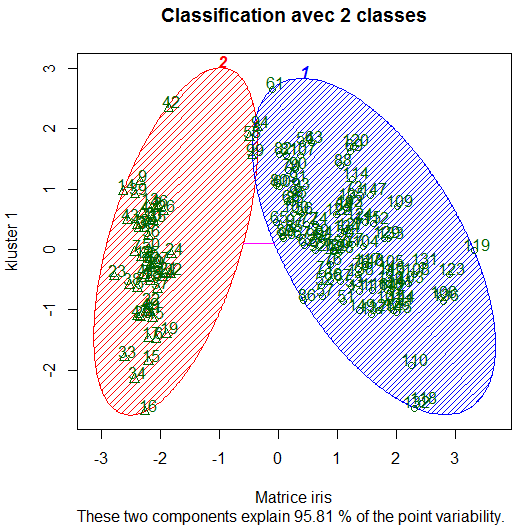
\includegraphics[height = 4.5cm, width = 4.5cm]{plots/2-2-1_kmeans.png}
      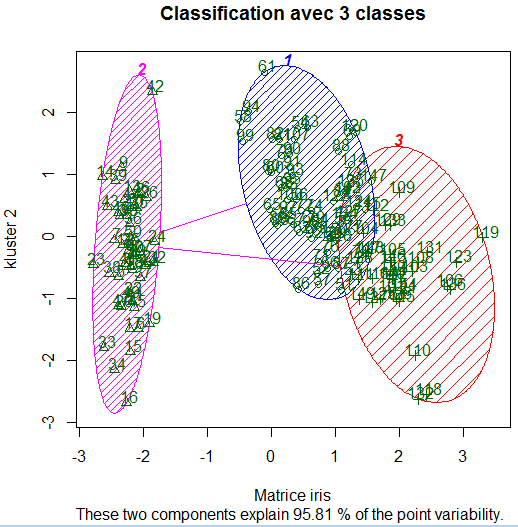
\includegraphics[height = 4.5cm, width = 4.5cm]{plots/2-2-2_kmeans.png}
      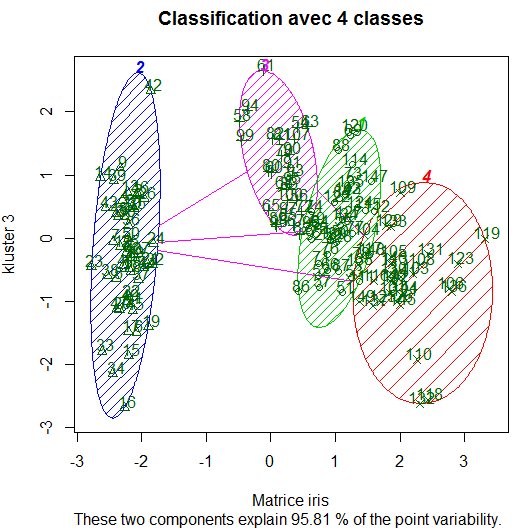
\includegraphics[height = 4.5cm, width = 4.5cm]{plots/2-2-3_kmeans.png}
    \end{center}
    
    \[\scriptsize{
    \begin{tabular}{|c|c|c|}
      \hline
       setosa & versicolor & virginica \\
      \hline
      0 & 47 & 50 \\
      \hline
      0 & 3 & 0 \\
      \hline
    \end{tabular}\ \
    \begin{tabular}{|c|c|c|}
      \hline
      setosa & versicolor & virginica \\
      \hline
      0 & 2 & 36 \\
      \hline
      50 & 0 & 0 \\
      \hline
      0 & 48 & 14 \\
      \hline
    \end{tabular}\ \
    \begin{tabular}{|c|c|c|}
      \hline
      setosa & versicolor & virginica \\
      \hline
      0 & 27 & 1 \\
      \hline
      0 & 23 & 17 \\
      \hline
      50 & 0 & 0 \\
      \hline
      0 & 0 & 32 \\
      \hline
    \end{tabular}
    }\]
    
    Nous pouvons noter lorsque $k=2$ l'ensemble de l’espèce $setosa$ est tout dans un seul cluster. En tant que les autres sont dans le deuxième. Nous pouvons remarquer que cela est du à que ces espèces ont une similarité plus grand entre elles que par rapport à l’espèce $setosa$.\\
    Nous avons constaté aussi que pour le cas où $k=4$, on a partitionné un quatrième groupe qui ni se différence pas trop des autres. Dans ce cas il possède environ 50\% de $versicolor$ et 50\% $virginica$. Donc nous avons conclu que n'est pas un groupe justifié et a été forcé pour l'algorithme pour son création. Alors pour $k=3$, nous avons constaté que le résultat est convenable et   plus propre que les autres obtenus. \\
    
  
  \item \textbf{Étude de la stabilité des partitions.}\\
  Pour interpréter la stabilité du résultat des partitions, on a réalisé une fonction qui a effectué la classification 50 fois au moyen de $kmeans$ dans 3 classes, et avec cela nous avons obtenu les valeurs de l'inertie intra-class, desquelles seulement ont lancé deux valeurs d'inerties différentes, 78,85144 et 142,75352. Cela nous indique que deux différentes classifications ont été obtenues. Celle de 78,85144 est de plus grande confiance, car l'inertie est plus basse. On en déduit que c'est la plus optimum.
Cette variation découle du fonctionnement de l'algorithme $kmeans$, qui prend comme référence une quantité g (classes) points au hasard pour générer les centres initiaux. Il y aura donc des variations dans les résultats.\\
Bien que la fonction n'est pas tout à fait stable, il existe une manière de réduire cette variabilité. On peut indiquer à l’algorithme le degré de variabilité des centres initiaux.\\

  
  \item \textbf{Détermination du nombre de classes optimal.}
    \begin{center}
      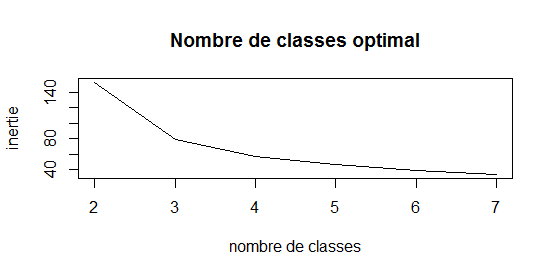
\includegraphics[height = 4.5cm, width = 8.5cm]{plots/2-3-a_classes.png}
    \end{center}
    Pour obtenir les valeurs de chaque inertie selon le nombre de classes, on a défini une fonction qui réalisait l'algorithme de classification \textit{kmeans 100 fois}, pour chaque nombre de classes.
On peut observer que la valeur d'inertie décroît par rapport à l'augmentation du nombre de classes. Cela découle du fait que plus il y a de classes, plus il y aura de centres de gravité, ce qui réduit la proximité des individus avec ces centres. Lorsque le nombre de classes tend vers la quantité d’individus dans le jeu de donnée l'inertie tendra à être nul.\\
Finalement, la méthode du coude nous aide à déterminer quel sera le nombre de classes. Au moyen de l'identification de l'abscisse, cela nous indique qu'il devrait y avoir 3 nombre de classes. Ce nombre correspond encore une fois au nombre d’espèces d’Iris. 
  
  
  \item \textbf{Comparaison des résultats des partitions réelles et l'obtenue par les centres mobiles}
    \begin{center}
      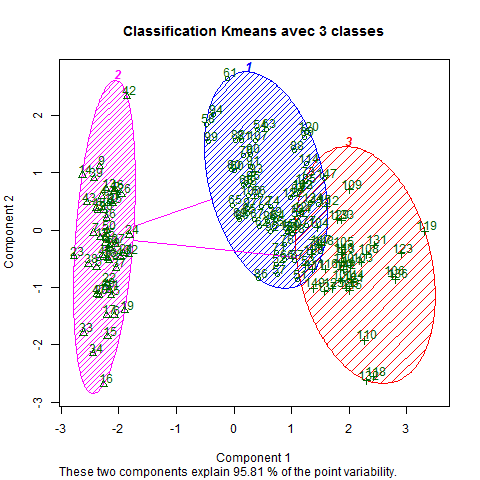
\includegraphics[height = 6.5cm, width = 6.5cm]{plots/2-4-1_clust_kmeans.png}
      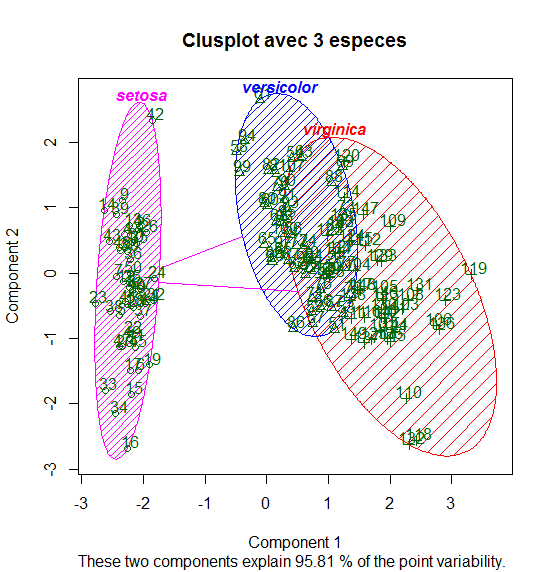
\includegraphics[height = 6.5cm, width = 6.5cm]{plots/2-4-1_clust_reelle.png}
    \end{center}
    \[\scriptsize{
      \hspace{1cm}
      \begin{tabular}{|c|c|c|}
  	  \hline
	    setosa & versicolor & virginica  \\
      \hline
      0 &  2 & 36  \\
      \hline
      50 &  0 & 0  \\
      \hline
      0 &  48 & 14  \\
      \hline
      \end{tabular}\hspace{1cm}
      \begin{tabular}{|c|c|c|c|}
	      \hline
	      & sectosa & versicolor & virginica \\
            \hline
            setosa &  50 & 0 & 0  \\
            \hline
            versicolor &  0 & 50 & 0  \\
            \hline
            virginica &  0 & 0 & 50  \\
            \hline
      \end{tabular}
      }\]
  Comme nous pouvons observer, le groupe deux obtenu par la méthode des centres mobiles, correspond à l’ensemble de l'espèce $setosa$. 
Le groupe trois est composé par 96\% des individus de $versicolor$ et de 28\% de $virginicas$. Le premier groupe reste presque représenté par l'espèce $virginica$, où seul 5,26\% correspondent à $versicolors$.

En général, on pourrait associer chaque classe à une espèce. Le premier groupe est l'espèce $virginica$, le deuxième les $setosa$, et le troisième $versicolor$, même s’il est composé à 20,59\% de $virginica$.


\end{enumerate}
\subsection{Donnés Crabs}
  \subsubsection{Comparaison des résultats des partitions réelles et l'obtenue par les centres mobiles}
    La quantité de classes convenables à choisir est égale à 4.
Ci-dessous les graphiques qui contiennent l’information obtenues à l’aide de la méthode des centres mobiles et de la partition réelle selon le sexe (H et F) et l’espèce (B et O) des crabes.
    \begin{center}
      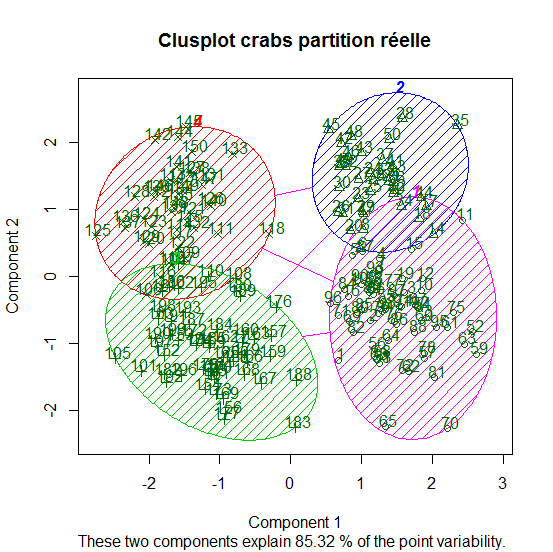
\includegraphics[height = 6.5cm, width = 6.5cm]{plots/2-4-2_crabs_kmeans.png}
      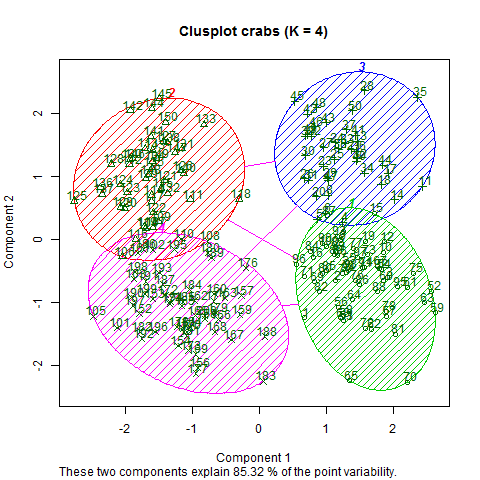
\includegraphics[height = 6.5cm, width = 6.5cm]{plots/2-4-2_crabs_reelle.png}
    \end{center}
    \[\scriptsize{
      \hspace{.5cm}
      \begin{tabular}{|c|c|c|c|c|}
	    \hline
	      F\&B & F\&O & M\&B & M\&O  \\
        \hline
        0 &  0 & 0 & 42  \\
        \hline
        0 &  49 & 0 & 8 \\
        \hline
        50 & 1 &  13 & 0  \\
        \hline
        0 & 0 &  37 & 0  \\
        \hline
      \end{tabular}\hspace{1.5cm}
      \begin{tabular}{|c|c|c|c|c|}
	      \hline
	        F\&B & F\&O & M\&B & M\&O  \\
          \hline
          0 &  0 & 0 & 38  \\
          \hline
          0 &  49 & 0 & 12 \\
          \hline
          50 & 1 &  16 & 0  \\
          \hline
          0 & 0 &  34 & 0  \\
          \hline
      \end{tabular}
      }\]
    On peut observer que les graphiques  sont similaires. Enfin, on peut déduire que la méthode des centres mobiles est d'une grande précision pour ce cas et elle nous pourvoit un résultat ajusté à la réalité de la situation.
\subsection{Donnés Mutations}
\subsubsection{kmeans, la stabilité du résultat de la partition.}
    \begin{center}
      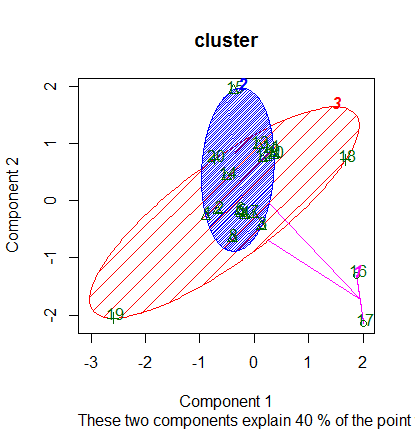
\includegraphics[height = 4.5cm, width = 4.5cm]{plots/graf1.png}
      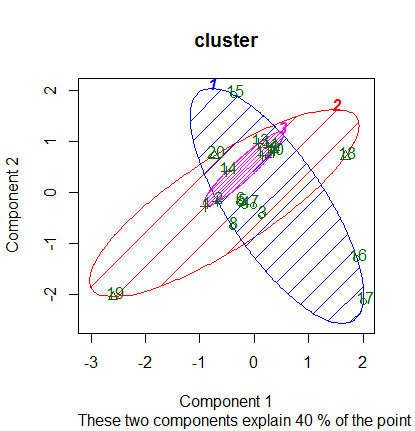
\includegraphics[height = 4.5cm, width = 4.5cm]{plots/graf2.png}
      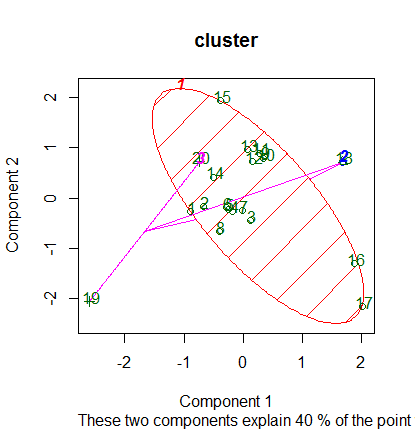
\includegraphics[height = 4.5cm, width = 4.5cm]{plots/graf3.png}
    \end{center}
Après d'avoir appliqué l'AFTD au tableau des distances mutation, nous avons fait 100 classifications sur les composantes principaux, ce que nous a donné plusieurs résultat différents. En observant la moyenne des inerties de chaque cluster. Et ces moyennes visent à être très proches  entre celles. Nous avons déduit que cela est à cause de la faible quantité des données, et donc ne permet pas de réussir à bien définir des clusters robustes.



\end{document}
